\section{Datenstrukturen}
\label{sec:datastructures}

%% Einführung in die übliche Arbeitsweise bei atomistischen Simulationen

Teilaspekte von Schichtabscheidungen wie Oberflächenreaktionen werden seit vielen Jahren erfolgreich mit KMC- und MD-Methoden simuliert\todo{refs}.
Zur Beschleunigung des Arbeitsablaufes kommt dabei häufig Standardsoftware zum Einsatz, die zwar für allgemeine Systeme optimiert wurde,
im Gegenzug allerdings für spezielle Probleme zu erhöhten Laufzeiten gegenüber spezialisierten Ansätzen führt.
Zu solchen Systemen zählen auch Oberflächenabscheidungen, die aufgrund ihrer geringen Dimensionalität (Oberflächen mit 2 effektiven Dimensionen), langen Laufzeiten (viele Millionen MD-Schritte) und additiver Arbeitsweise (Schrittweises Hinzufügen einzelner Atome) stark von speziellen Optimierungen profitieren können.

%% Vorteile von und Vorgehensweise für Expertensysteme

Die Unterschiede zwischen der Betrachtung allgemeiner und spezieller Systeme liegen dabei in den genutzten Algorithmen und Datenstrukturen:
Bessere Systemkenntnis ermöglicht eine genauere Abschätzung der Häufigkeit bestimmter Operationen, und somit die Wahl und Anpassung von Algorithmen auf die Klasse der zu untersuchenden Systeme.
Dafür werden die Vor- und Nachteile in Form der asymptotischen Laufzeiten von Operationen gegenüber deren Häufigkeit und Speicherverbrauch der Datenstruktur abgewogen.
Als Resultat werden häufige Operationen beschleunigt, wodurch die Effizienz der gesamten Simulation gesteigert und größere Systeme ermöglicht werden.
Es bleibt zu erwähnen, dass der Speicherverbrauch bei den auf das Problem anwendbaren Datenstrukturen linear mit der Systemgröße skaliert, weshalb der primäre Engpass in der Rechenzeit und nicht im Speicherverbrauch liegt.

\subsection{Systemeigenschaften}

Bei den zu betrachtenden Systemen handelt es sich um atomistische Bulks und Oberflächen ohne explizite Simulation der Gasphase.
Für diese ergeben sich folgende Eigenschaften:
\begin{enumerate}
\item Lokalität\\
  Interatomare Einflüsse sind reichweitenbegrenzt
\item Niedriger Diffusionskoeffizient\\
  Atome behalten ihre Nachbarschaft für relativ lange Zeiträume bei
\item Scharfe Oberflächen\\
  Die Oberfläche des Systems ist eindeutig durch eine Menge von Atomen festgelegt
\item Gleichverteilung der Teilchendichte\\
  Es lässt sich eine untere und obere Grenze für Nächstnachbarabstände angeben
\item Teilweise Periodizität\\
  Betrachtete Systeme können entlang ausgewählter Hauptachsen periodisch sein
\end{enumerate}

Einzig das Diffusionskriterium ergibt sich aus der Notwendigkeit, Atompositionen über einen langen Zeitraum ohne Manipulation effizient zu speichern.
Man könnte Diffusionen jedoch auf verschiedene Arten in das Parsivald-Modell einarbeiten.
Dazu zählen explizite MD-Simulationen der Oberfläche ebenso wie Monte-Carlo-Simulationen der Position von Oberflächen- oder Bulkteilchen.
Im Rahmen dieser Arbeit möchte ich zuerst auf diffusionsarme Materialien und Precursorsysteme zurück greifen, bevor der allgemeine Fall betrachtet wird.

Als Resultat der oben genannten Systemeigenschaften lassen sich Annahmen für dir algorithmische Betrachtung des Systemes treffen.
Beispiele solcher Annahmen, die in der Umsetzung des Parsivald-Modelles relevant wurden, zeigt folgende Liste.

\begin{enumerate}
\item Reaktionssimulationen sind auch auf Ausschnitte der Gesamtstruktur durchführbar
\item Nachbarschaftslisten müssen selten aktualisiert werden\\
  Die Reichweite einer Manipulation ist begrenzt
\item Oberflächenatome befinden sich zu einander in direkter Nachbarschaft
\item Die Zahl der Nachbarn unterliegt einer oberen Schranke
\item Divide-and-Conquer-Algorithmen müssen aufwendigeres Stitching betreiben
\end{enumerate}

Ohne diese Annahmen stellten einige der ausgewählten Operationen das System nur unzureichend dar.

\subsection{Benutzte Operationen}

\begin{table}[b]
  \caption[datasymbols]{Symbole für Laufzeit- und Speicherabschätzungen}
  \label{tab:datasymbols}
  \begin{tabularx}{\textwidth}{|lX|lX|}
    \hline
    {Symbol} & {Bedeutung} & {Symbol} & {Bedeutung} \\
    \hline
    \BigO{expr} & Worst-Case-Komplexität & $n$ & Zahl der Atome \\
    $k$ & Zahl von Nächstnachbarn & $b$ & Zahl der Bins \\
    $k_r$ & Zahl von Nachbarn mit $d \leq r_c$ & $r_c$ & Cutoff-Radius \\
    $r_s$ & Suchradius & $s$ & lineare Raumgröße \\
    \hline
  \end{tabularx}
\end{table}

\todo[inline]{Referenzen der optimalen Laufzeiten!}

Aus Sicht der aufrufenden Simulation ist die Wahl der unterliegenden Datenstruktur nicht ersichtlich.
Für sie besteht die Interaktion aus Operationen, die auf die Menge von Atomen ausgeführt werden.
Das beinhaltet Konstruktions-, Manipulations- und Suchoperationen auf dieser Menge.
Ein Vergleich der asymptotischen Laufzeiten ist in Tabelle \ref{tab:dataruntimes} dargestellt.

\subsubsection{Konstruktion}
Damit wird der einmalige Aufbau der gesamten Struktur aus einer beliebigen Menge von Atomen bezeichnet.
Dadurch steht die eigentliche Laufzeit dieser Operation im Hintergrund.

Liegt kein separater Algorithmus vor, kann die Struktur durch iterative Einfügung einzelner Atome angenähert werden, und verhält sich somit linear zur Laufzeit der Einfügungsoperation, und somit maximal quadratisch zur Zahl der Atome.
Optimal ist hier \BigO{n} bei simplen Listen, im Gegensatz zu \BigO{n^2} bei Nachbarschaftslisten\ref{}.

\subsubsection{Einfügung}
Je nach Datenstruktur auch Push-Operation genannt, bezeichnet sie das Einfügen eines neuen Atomes in eine bestehende Struktur.
Dies geschieht im Parsivald-Modell nach erfolgreichen Reaktionen von Gasmolekülen auf der Oberfläche, bei denen die neu aufgebrachten Atome dem Simulationsraum beigefügt werden.
Da diese Operation vergleichsweise häufig aufgerufen wird, bieten sich Strukturen an, bei denen nur die lokale Nachbarschaft, nicht aber die gesamte Struktur aktualisiert werden muss.

Optimale Laufzeit ist das Hinzufügen eines Atomes an das Ende einer Liste in konstanter Zeit (\BigO{1}), jedoch verlangen einige Strukturen den Vergleich mit allen anderen Atomen, wodurch sich \BigO{n} ergibt.

\subsubsection{Modifikation}
Auch als Up\-date-Operation bekannt, führt sie eine Aktualisierung der Positionen oder des Typen\footnote{Einige Anwendungen erfordern die separate Betrachtung verschiedener Adsorptions- oder Oxidationszustände durch separate Atomtypen} einzelner oder mehrerer Atome durch.

Auch hier lässt sich konstante Zeit als Optimum angeben, wo hingegen beispielsweise Nachbarschaftslisten komplett neu aufgebaut und somit Laufzeitgrenzen von \BigO{n} angegeben werden müssen.

\subsubsection{Entfernung}
Als Gegenstück zur Push-Operation entfernt diese eines oder mehrere Atome aus dem Simulationsraum.
Diese Operation wird angewandt, wenn durch Reaktionen einzelne Liganden von der Oberfläche entfernt werden und findet somit Anwendung bei Simulationen, die den gesamten Precursor betrachten.
Es gelten die gleichen Laufzeitgrenzen wie bei der Einfügung von Atomen.

\subsubsection{Nachbarschaftssuche}
Ihrem Namen entsprechend sucht diese Operation nach allen Atomen in der Nachbarschaft eines vorher bekannten Atomes.
Sie wird beim Parsivald-Modell genutzt, um die lokale Nachbarschaft eines Referenzatomes für eine MD-Simulationen zu extrahieren, und somit bei jedem ausgewählten KMC-Ereignis ausgeführt.

Die Laufzeit variiert stark zwischen \BigO{1} für Nachbarschaftslisten, die die Komplexität in die anderen Operationen auslagern, und \BigO{n}, falls die Position aller Atome explizit verglichen werden muss.
Häufig ist die Laufzeit auch proportional zur oberen Grenze der Zahl von Nachbarschaftsatomen und somit zum kubischen Suchradius.

\subsubsection{Ortssuche}
Im Unterschied zur Nachbarschaftssuche sucht man hier alle Atome im Umkreis eines beliebigen Punktes im Raum.
Diese Operation wird zur Identifizierung eines Reaktionsortes und somit zum Aufbau eines KMC-Ereignisses genutzt.
Damit ist sie die häufigste Operationen und sollte im Mittelpunkt von Optimierungsbemühungen stehen.
Da beide Nachbarschaftssuchen in einander überführbar sind, ist ihre Komplexität mit wenigen Ausnahmen gleich.

\subsubsection{Oberflächensuche}
Diese Operation sucht die Oberfläche, entweder entlang einer definierten Geraden oder im Umkreis eines Punktes.
Die Art der Eingangsgröße kann von der aufrufenden Simulation zugunsten der Laufzeit gewählt werden.

Hier bietet die Delaunay-Triangilation die besondere Eigenschaft, die Oberfläche eines Systems direkt ermitteln und in der Datenstruktur speichern zu können.
Sie ist dann für den KMC-Teil der Simulation durch eine Menge von Oberflächenatomen charakterisiert, die sich mit jeder Schreiboperation auf der Struktur automatisch aktualisiert.
Auch die Oberflächennormale ist dabei gegeben, ohne zusätzliche komplizierte Prüfungen anstellen zu müssen, so dass man beispielsweise Auftreffwahrscheinlichkeiten für KMC-Ereignisse ohne weiteres berechnen kann.
Dafür muss man im Gegenzug den KMC-Algorithmus auf Zusammenarbeit mit der Triangulation anpassen, anstatt einen abstrakten Algorithmus mit expliziten Oberflächensuchen nutzen zu können.
Aus diesen Gründen nehme ich die Komplexität im Rahmen der kombinierten KMC-MD-Simulation mit \BigO{1} als konstant an, obwohl eine explizite Oberflächensuche eine superlogarithmische Laufzeit hätte.

\begin{table}[hb]
  \centering
  \begin{tabularx}{\textwidth}{X|*8c}
    Datenstr.  &  Konstr.          &  Einfüg.          &  Modif            &  Entf.            &  Ortss.                      &  NB-Su.               &  Oberfl.         &  RAM                          \\
    \hline
    Atomlisten  &  \cG{$n$}         &  \cG{$1$}         &  \cG{$1$}         &  \cG{$1$}         &  \cR{$n$}                    &  \cR{$n$}             &  \cR{$n$}        &  \cG{$n$}                     \\
    NB-Listen  &  \cY{$n\log{n}$}  &  \cR{$n$}         &  \cR{$n$}         &  \cR{$n$}         &  \cR{$n$}                    &  \cG{$1$}             &  \cR{$n$}        &  \cR{$\frac{r_c^3}{s^3}n^2$}  \\
    Binning    &  \cG{$n$}         &  \cG{$1$}         &  \cG{$1$}         &  \cG{$1$}         &  \cG{$r_s^3$}                &  \cG{$r_s^3$}         &  \cR{$c$}        &  \cY{$n+c$}                   \\
    Octree     &  \cY{$n\log{c}$}  &  \cY{$\log{c}$}   &  \cY{$\log{c}$}   &  \cG{$1$}         &  \cY{$r_s^3\log{c}$}         &  \cY{$r_s^3\log{c}$}  &  \cY{$\log{c}$}  &  \cY{$n+c^\frac{2}{3}$}       \\
    k-d-Baum   &  \cY{$n\log{n}$}  &  \cY{$\log{n}$}   &  \cY{$\log{n}$}   &  \cY{$\log{n}$}   &  \cY{$r_s^3\log{n}$}         &  \cY{$r_s^3\log{n}$}  &  \cY{$\log{n}$}  &  \cG{$n$}                     \\
    Delaunay   &  \cY{$n\log{n}$}  &  \cY{$k\log{k}$}  &  \cY{$k\log{k}$}  &  \cY{$k\log{k}$}  &  \cG{$r_s^3+n^\frac{1}{3}$}  &  \cG{$r_s^3$}         &  \cG{$1$}        &  \cY{$nk$}                    \\
    \hline
    %Atomfeld  &  \cG{$n$}         &  \cG{$1$}         &  \cG{$1$}         &  \cG{$1$}         &  \cR{$n$}                    &  \cR{$n$}             &  \cR{$n$}        &  \cG{$n$}                     \\
  \end{tabularx}
  \vspace{1em}
  \begin{tabularx}{0.8\textwidth}{C*3C}
    &\cG{optimal} & \cY{annehmbar} & \cR{impraktikabel} \\
  \end{tabularx}
  \caption[Laufzeitabschätzung abstrakter Operationen auf verschiedenen Datenstrukturen]{
    Abschätzung des Speicheraufwands und der asymptotischen Laufzeit der vorgestellten Operationen auf verschiedenen Datenstrukturen für kompakte Oberflächensysteme in drei Raumdimensionen.
    \todo[inline]{Referenzen oder Erklärungen}.
  }
  \label{tab:dataruntimes}
\end{table}

\subsection{Kategorien von Datenstrukturen}

Durch Unterschiede in der Funktionsweise verschiedener Algorithmen und Datenstrukturen ergeben sich für sie Kategorien, die generelle Eigenschaften wie die Laufzeit teilen.
Während der Entwicklung und Implementierung des Parsivald-Modelles wurden Algorithmen aus den folgenden Kategorien in Betracht gezogen.

\subsubsection{Listen}

Listen von Atomen sind die einfachste Datenstruktur zur Behandlung von Punktwolken, da sie neben den Atompositionen, -typen und einer beliebigen Laufnummer keine weiteren Informationen beinhalten.
Die einzelnen Atome werden in einer globalen Liste verwaltet, wodurch Manipulationsoperationen in optimaler konstanter Zeit möglich sind, Nachbarschaftsoperationen und Positionsvergleiche andererseits Vergleiche mit sämtlichen Atomen benötigen und somit die Worst-Case-Laufzeit von \BigO{n} annehmen.

Für große Systeme sind listenbasierte Ansätze folglich ungeeignet, wie man an deren Laufzeiten in Tabelle \ref{tab:dataruntimes} erkennen kann.

\subsubsection{Nachbarschaftslisten}

Nachbarschaftslisten sind eine Form von Atomlisten, die zusätzlich zur Position jedes Atoms auch eine Liste von Referenzen auf alle Atome in dessen Nachbarschaft speichern.
Diese müssen aber bei jeder Manipulation aufwendig aktualisiert werden, wodurch im Gegenzug die Nachbarschaftssuche in konstanter Zeit \BigO{1} möglich ist.
Für MD-Simulationen mit reichweitenbegrenzten Kraftfeldern bieten sich Nachbarschaftslisten zur signifikanten Reduktion der Programmlaufzeit an.
Dabei muss erwähnt werden, dass einige der \BigO{n}-Operationen durch geeignete Optimierungen auf Laufzeiten von \BigO{rk} reduzieren lassen, jedoch basieren diese meist auf häufigen Aktualisierungen bei geringen relativen Atombewegungen.
Unterliegen die Positionsänderungen größeren Schritten, wie es beim Parsivald-Modell durch seine separaten atomistischen Simulationen der Fall ist, ergeben sich grenzwertig wieder \BigO{n}-Abhängigkeiten.

\subsubsection{Binning}

Eine implizite Möglichkeit, die lokale Nachbarschaft zu referenzieren, findet man in Binning-Methoden, die die Zuordnung von räumlichen Positionen in meist quaderförmige Raumbereiche, Bins genannt, umfassen.
Dafür zerlegt man den Raum in kleinere, leicht addressierbare Quader, für die man Listen der enthaltenen Atomepflegt, die nur noch bei Überschreitung der Quadergrenzen aktualisiert werden müssen.
Die Nachbarn ergeben sich dann aus einer Suche innerhalb der benachbarten Quader in Abhängigkeit des Suchradius', wobei periodische Systemgrenzen durch relative Addressierung der Bins elegant versteckt werden.

Die Bins selbst lassen sich nun wiederum in Listen, mehrdimensionalen Gittern oder Baumstrukturen speichern, wobei jede Methode ihre eigenen Vor- und Nachteile hat.
Im Rahmen der Arbeit wurden hauptsächlich Octrees genutzt, wie sie in Abschnitt \ref{dataoctree} beschrieben werden.

\begin{figure}[bhpt]
  \captionsetup[subfigure]{singlelinecheck=false}{
    \def\subfigwidth{0.23\textwidth}
    \def\svgwidth{\textwidth}
    \begin{subfigure}[t]{\subfigwidth}
      \includegraphics[width=\textwidth]{datastructures-a}
      \subcaption{Ohne Binning}
      \label{fig:datastructures-a}
    \end{subfigure}
    \hfill
    \begin{subfigure}[t]{\subfigwidth}
      \includegraphics[width=\textwidth]{datastructures-b}
      \subcaption{Binning}
      \label{fig:datastructures-a}
    \end{subfigure}
    \hfill
    \begin{subfigure}[t]{\subfigwidth}
      \includegraphics[width=\textwidth]{datastructures-c}
      \subcaption{Octree}
      \label{fig:datastructures-a}
    \end{subfigure}
    \hfill
    \begin{subfigure}[t]{\subfigwidth}
      \includegraphics[width=\textwidth]{datastructures-d}
      \subcaption{k-d-Baum}
      \label{fig:datastructures-a}
    \end{subfigure}
  }
  \caption[Übersicht über räumliche Datenstrukturen]{
    Übersicht über Raumzerlegungen einiger Datenstrukturen.
    k-d-Bäume (d) beinhalten in jeder Zelle nur ein Atom, weshalb sich die Zellgrenzen entlang der Atompositionen formen.
    Octrees (c) dagegen haben vordefinierte Grenzen, aber prägen nur besetzte Zellen aus, wodurch leere Raumbereiche effizient von Suchoperationen ausgeschlossen sind.
}
  \label{fig:datastructures}
\end{figure}

\subsubsection{Suchbäume}

Eine andere Möglichkeit, Bäume für die Optimierung von Suchfunktionen zu nutzen, findet sich in k-dimensionalen Bäumen, auch k-d-Bäume genannt.
Diese sind rekursive Datenstrukturen, die alle Atome entlang einer Hauptachse sortieren, das Median-Element als Root-Knoten herausnehmen und jeweils aus den beiden verbleibenden Atommengen einen neuen k-d-Baum entlang der zyklisch nächsten Hauptachse aufbauen.
Der Hauptnutzen dieses Ansatzes findet sich in vereinfachten Nachbarschafts- und Ortssuchen, die jeweils in \BigO{k_r\log{n}} möglich sind, was bei den untersuchten Systemen \BigO{r_s^3\log{n}} entspricht.
Da es sich bei k-d-Bäumen um einen Lehrbuchansatz bei Nachbarschafts- und Suchproblemen handelt, werden sie nachfolgend in Abschnitt \ref{datakdtree} eingehender beschrieben.

\subsubsection{Triangulationen}

Triangulationen kann man als eine spezielle Form von Nachbarschaftslisten betrachten, bei denen ausgeprägte Nachbarschaftsbedingungen besonderen Kriterien unterliegen.
Sie zerlegen die konvexe Hülle der Punktwolke in eine Menge von raumfüllenden, nicht-überschneidenden $k$-Simplexen\footnote{Ein $k$-Simplex ist ein Objekt in $k$ Dimensionen mit $k+1$ Eckpunkten, die untereinander mit geraden Kanten verbunden sind. Somit ist ein 1-Simplex eine Linie, ein 2-Simplex ein Dreieck, ein 3-Simplex ein Tetraeder, usw.}, deren Ecken auf Elementen der Punktwolke liegen.
Damit teilen sich alle Atome mindestens einen Simplex mit ihrem nächsten Nachbarn, jedoch nicht notwendigerweise mit allen Nachbarn innerhalb eines bestimmten Radius'.
Für Triangulationen gibt es verschiedene Ausprügungen der Kriterien, wobei in dieser Arbeit die populäre Delaunay-Triangulation aufgrund ihrer Dualität zu Voronoi-Diagrammen und der direkten Verbindung zur Alpha-Form in Abschnitt \ref{datadelaunay} betrachtet wird.

\subsection{Effiziente Datenstrukturen}

Zur Betrachtung der in Abschnitt \ref{sec:parsivald} vorgestellten Problemstellungen bieten sich nur eine Auswahl der angesprochenen Datenstrukturen an, da die asymptotischen Laufzeiten der Suchoperationen auf den ausgeschlossenen Strukturen oberhalb der Praktikabilitätsgrenze liegen.
Als Auswahl effizienter Datenstrukturen werden weiterhin Octrees, k-d-Bäume und Delaunay-Triangulationen behandelt.

\subsubsection{Octrees}\label{dataoctree}
Octrees können als Optimierungen für Binning-Methoden genutzt werden, indem man die Zellen in einem Suchbaum statt in Zellgittern organisiert.
Dazu wird der Simulationsraum rekursiv in 8 geometrisch ähnliche Unterzellen halber Breite aufgeteilt, bis die gewünschte Auflösung erreicht ist.
Als Vorteil ergeben sich die ausschließliche Erstellung für die Simulation relevanter Unterzellen, sowie die Betrachtung leerer Raumbereiche als zusammengefasste Superzelle, wie in Abbildung \ref{fig:octree} dargestellt.
Resultat sind verringerter Speicherbedarf und beschleunigte Suchoptionen, die irrelevante Gebiete schneller überspringen können.

Theoretisch sind mit Access Caching, Bitweiser Addressierung, Surface Flagging oder Height Mapping noch weitere Anpassungen möglich, allerdings verbessert sich dabei nur der Laufzeitfaktor, nicht die asymptotische Laufzeit, weshalb sie nur am Rand genannt sein sollen.
Algorithmus \ref{algo:octreeaddressing} skizziert die Addressierung der Zelle eines Octrees und zeigt auch deren Schwachpunkt:
Um eine einzige Zelle per absolutem oder relativem Index abzurufen, sind Operationen der Komplexität \BigO{\log{c}} notwendig, die bei häufigen Zellzugriffen und großen Systemen sowie kleinen Zellen zu Leistungseinbrüchen führen können.

%% \begin{algorithm}
%%   \begin{algorithmic}
%% %    \Input $atoms$ - Liste der Atome
%% %    \Input $size[3]$ - Größe des Simulationsraumes
%% %    \Input $depth$ - Tiefe des Octrees (Legt die Zellgröße fest)
%% %    \Assumption Alle Atome befinden sich im Simulationsraum
%% %    \Result Stammzelle eines Octrees, der alle Atome enthält
%%     \State
%%     \Function{construct-octree}{$atoms, spacesize, depth$}
%%     \State $cellsize[0] \gets spacesize[0]\cdot2^{-depth}$
%%     \State $cellsize[1] \gets spacesize[1]\cdot2^{-depth}$
%%     \State $cellsize[2] \gets spacesize[2]\cdot2^{-depth}$
%%     \State $root \gets$ new Octree($depth$)
%%     \ForAll{$atom$ in $atoms$}
%%     \State $cellindex[0] \gets \lfloor atom.pos[0] / cellsize[0] \rfloor$
%%     \State $cellindex[1] \gets \lfloor atom.pos[1] / cellsize[1] \rfloor$
%%     \State $cellindex[2] \gets \lfloor atom.pos[2] / cellsize[2] \rfloor$
%%     \State $cell \gets$ \Call{getcell-octree}{$root, cellindex$, true}
%%     \State \Call{add-atom}{cell, atom}
%%     \EndFor
%%     \State \Return $root$
%%     \EndFunction
%%   \end{algorithmic}
%%   \caption[Octree-Konstruktion]{Octree-Konstruktion: Es handelt sich um einen typischen Binning-Algorithmus, dessen Octree-Eigenschaften in der Funktion \Call{getcell-octree}{} liegen.}
%%   \label{alco:octree-construction}
%% \end{algorithm}

\begin{figure}[tbhp]
  \centering
  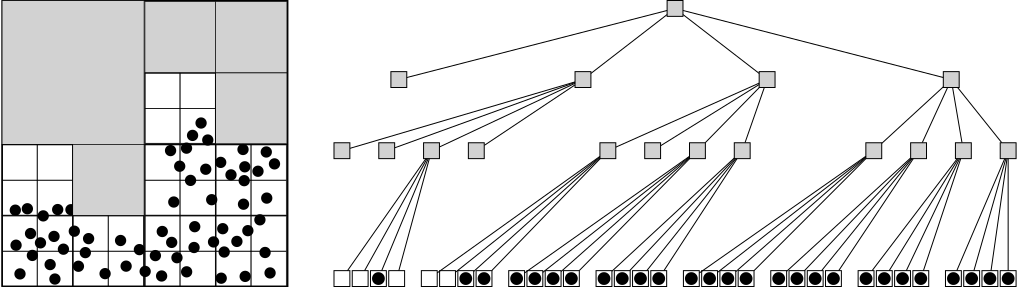
\includegraphics[width=\textwidth]{octree}
  \label{fig:octree}
  \caption[Funktionsweise eines Octrees]{Quadtree (2d-Äquivalent des Octrees) zur Veranschaulichung der Funktionsweise eines Octrees:
    Räumliche Unterteilung und deren die Baum-Darstellung.
    Rekursive Zerlegung der interessanten Zellen bis zur gewünschten Auflösung in Ebene 4, dann zellweises Binning der Atome.
  }
\end{figure}

\begin{algorithm}
  \begin{algorithmic}
%    \Input $root$ - Stammzelle des Octrees
%    \Input $i[3]$ - globale Adresse der Zielzelle
%    \Input $allocate$ - Ob die Zelle neu erstellt werden soll
    \Result null falls leer, sonst Zielzelle
    \State
    \Function{getcell-octree}{$cell, id, allocate$}
    \State $d \gets $\Call{depth}{root}
    \Comment{Relative Tiefe, an der sich die Zielzellen befinden}
    \If{$d = 0$}
    \State\Return cell
    \EndIf
    \If{not $cell.children$}
    \If{allocate}
    \State $cell.children \gets $new cell[8]
    \Else
    \State \Return null
    \EndIf
    \EndIf
    \State $childid \gets $\Call{bitand}{id[0], $2^{d-1}$}
    + $2\cdot$\Call{bitand}{id[1], $2^{d-1}$}
    + $4\cdot$\Call{bitand}{id[2], $2^{d-1}$}
%    \State \Comment{Indiziert die Subzelle aus der globalen Position}
    \State \Return\Call{getcell-octree}{$cell.children[childid], i, allocate$}
    \EndFunction
  \end{algorithmic}
  \caption[Zell-Addressierung in Octrees]{Rekursive Zell-Addressierung und -Allokierung im Octree: Bei jedem Schritt wird das Problem in 8 Unterzellen geteilt, woraus eine Laufzeit von \BigO{d}$=$\BigO{\log{c}} resultiert}
  \label{algo:octreeadressing}
\end{algorithm}

\todo[inline]{Wars das? Formeln?}

\subsection{k-d-Bäume}

Für Nachbarschafts- und Bereichssuchen wird wegen ihrer hervorragenden Suchkomplexität auf k-d-Bäume zurückgegriffen, die einen kartesischen Raum in orthogonale Zellen mit jeweils einem Atom unterteilen.
Es ergibt sich ein balancierter Binärbaum mit Atomen als Knoten, dessen Haupteigenschaft in impliziter Betrachtung von Abstandsrelationen liegt.
So lassen sich große Bereiche aus einer Abstandssuche oder Bereichssuche ausschließen, sobald ein Atom mit geringerem Abstand gefunden wurde.
Somit lässt sich per binärer Suche das nächste Atom eines beliebigen Punktes in \BigO{\log{n}} finden.
Sucht man $N$ Nächstnachbaratome, lassen sie sich durch Kombination mit einem Heap in \BigO{\log{n}\log{N_r}} finden, was zwar im Vergleich zu Octrees zu höheren asymptotischen Laufzeiten führt, jedoch zu kürzeren realen Laufzeiten führt.
\footnote{Vergleich dazu auch Heapsort vs. Quicksort: Cachingeffekte}
Aktualisierungen von Knoten behandelt man durch Standardalgorithmen wie Baumrotation in \BigO{\log{n}}.

Eine weitere Eigenschaft von k-d-Bäumen ist außerdem, dass sie nicht auf endliche Räume beschränkt sind und zuverlässig beliebig große Systeme beschreiben können.
Durch adaptives Neubalancieren erreicht man dennoch bei typischerweise einseitigem Schichtwachstum die oben erwähnten Suchlaufzeiten auf Kosten der Manipulationseffizienz.

\begin{figure}[bthp]
  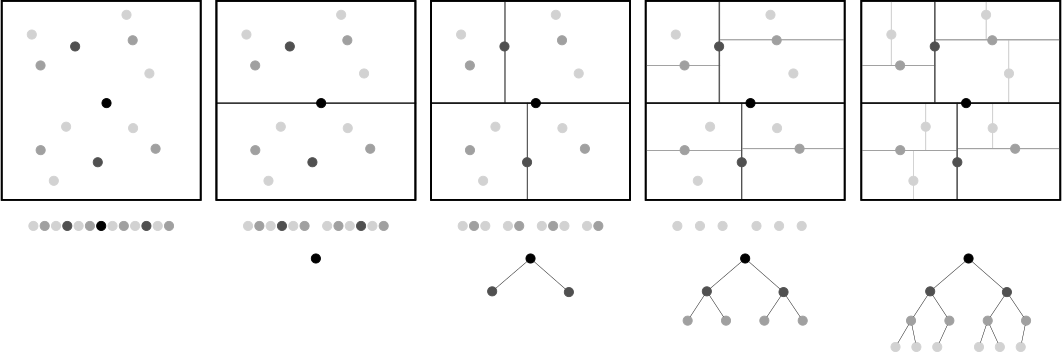
\includegraphics[width=\textwidth]{kdtree-tree}
  \caption[Konstruktion eines k-d-Baumes]{
    Rekursive Konstruktion eines k-d-Baumes: Die Punktmenge wird sortiert, der Median zum Baum hinzugefügt und seine Kinder aus den beiden Teilmengen per k-d-Baum-Konstruktion gewonnen.
    Der gewonnene Suchbaum ist effizient in Speicherplatz und Laufzeit der Suchoperationen.
  }
  \label{fig:kdtree}
\end{figure}

%% \begin{algorithm}
%%   \begin{algorithmic}
%%     \Input $points$ - Liste von Punkten
%%     \Input $k$ - Dimensionalität des Simulationsraumes
%%     \Result Root-Element eines vollständigen KD-Baumes aus diesen Punkten
%%     \State
%%     \Function{construct-kdtree}{$points, dim\gets0$}
%%     \State $n\gets$\Call{length}{points}
%%     \If{$n=0$}
%%     \State \Return null
%%     \Else
%%     \State \Call{sort}{$points, dim$} \Comment{Sortiert $points$ nach pos[$dim$]}
%%     \State $root\gets{}points\left[\lfloor\frac{n}{2}\rfloor\right]$
%%     \State $dim\gets(dim+1)\mod{k}$
%%     \State $root.left \gets$ \Call{construct-kdtree}{$points\left[0:\lfloor\frac{n}{2}\rfloor-1\right], dim$}
%%     \State $root.right \gets$ \Call{construct-kdtree}{$points\left[\lfloor\frac{n}{2}\rfloor+1:n-1\right], dim$}
%%     \State \Return $root$
%%     \EndIf
%%     \EndFunction
%%   \end{algorithmic}
%%   \caption[Konstruktion eines k-d-Baumes]{Rekursive Konstruktion eines k-d-Baumes (naive Implementierung)}
%%   \label{algo:kdtree-construction}
%% \end{algorithm}

Probleme von k-d-Bäumen zeigen sich bei der Suche nach einer Oberfläche einerseits und bei periodischen Räumen andererseits.
Die Oberfläche entlang einer Hauptachse lässt sich per Range Search mit anschließender Minimalsuche entlang der Suchachse effizient ermitteln, möchte man allerdings das Auftreffen eines Precursors mit beliebiger Inklination ermitteln, kann man auf keine optimale Methode zurückgreifen, sondern muss die Range Search auf einen größeren orthogonalen Suchbereich erweitern und darin eine Auswahl treffen.
Zudem führen lokale Aktualisierungen im schlimmsten Fall zur Neubalancierung des gesamten Baumes, wodurch die Betrachtung paralleler verzögerter Aktualisierungen erschwert wird.
Periodische Simulationsräume führen außerdem in der Nähe der Systemgrenze zu identischen Operationen auf periodischen Bildern des Baumes, die bei eventuellen Aktualisierungen ebenso weitreichende Restrukturierungen zur Folge haben.

Aus diesen Gründen lassen sich k-d-Bäume nicht zufriedenstellend im Parsivald-Modell nutzen.

\subsection{Delaunay-Triangulation}\label{datadelaunay}

\begin{figure}[bhpt]
  \centering
  \def\svgwidth{\textwidth}
  \input{img/delaunay.pdf_tex}
  \caption[Delaunay-Triangulation]{Beispiel der Konstruktion einer Delaunay-Triangulation (c) aus einer Punktwolke (a).
    Für jedes Simplex (hier 2d-Simplex, also Dreieck) muss das Delaunay-Kriterium eingehalten werden:
    Es dürfen sich keine weiteren Punkte im Umkreis des Simplices befinden (b).
  }
  \label{fig:delaunay}
\end{figure}

Eine alternative Partitionsmethode findet sich in Triangulationen, die die konvexe Hülle der Punktwolke raumfüllend in nichtüberlappende k-dimensionale Simplexe entsprechend einer weiterhin Delaunay-Kriterium genannten Beziehung zerlegen:
Im Umkreis eines Simplexes befinden sich keine weiteren Punkte aus der Punktwolke.
Damit ergibt sich eine Vielzahl an Eigenschaften, die für verschiedene Problemstellungen zu effizienten Lösungen führen.
So beinhaltet eine Delaunay-Triangulation als Subgraphen den Nächstnachbargraphen, die Alpha-Form und die konvexe Hülle, ist dual zum Voronoi-Diagramm und es lässt sich leicht auf Konnektivität prüfen.


\begin{itemize}
\item Jeder Punkt ist Eckpunkt eines oder mehrerer Simplexe
\item Simplexe überschneiden sich nicht
\item Im Umkreis eines Simplexes befinden sich keine weiteren Punkte
\item Die Vereinigung aller Simplexe ergibt die konvexe Hülle
\item Alpha-Form $\subset$ Delaunay-Triangulation
\item %Ein Punkt teilt sich mit seinem nächsten Nachbarn mindestens einen Simplex \\
  %$\Leftrightarrow$
  Nächstnachbargraph $\subset$ Delaunay-Triangulation
  %% \item Die Delaunay-Triangulation und das Voronoi-Diagramm über die selben Punkte sind dual\\
  %% $\Rightarrow$ Allgemeine Nachbarschaftssuche ist \BigO{k\log k}
\end{itemize}

Delaunay-Triangulationen werden somit für Oberflächenbetrachtungen interessant, da sie über die Alpha-Form, welche durch Auswahl der Punkte aller Simplexe mit Umkreisradien oberhalb einer stoffabhängigen Grenze ermittelt wird und die wahrgenommene Oberfläche eines Systems darstellt.
Somit lassen sich Oberflächenrauheiten, Nanoporen und bei extremen Grenzwerten auch Kristalldefekte bestimmen.
Mit wenig Mehraufwand gegenüber reinen Delaunay-Triangulationen ließen sich somit einerseits Auswertungen bei laufenden Simulationen durchführen und Prozesse gegebenenfalls direkt optimieren, andererseits ist die gesamte Oberfläche zur Simulation von Oberflächenereignissen bekannt und direkt parametrisiert.

\subsubsection{Algorithmen zur Konstruktion einer Delaunay-Triangulation}

Zur Delaunay-Triangulierung aus einer Punktmenge stehen verschiedene Algorithmen zur Verfügung, die auf unterschiedlichen Methoden aufbauen.

\begin{itemize}
\item Flip-basierte Algorithmen (Local Improvement)\\
  Man startet mit einer beliebigen Triangulation, prüft den Umkreis aller Simplexe auf enthaltene Punkte und korrigiert gegebenenfalls per Flip-Algorithmus, der in Abbildung \ref{fig:delaunay-flip} dargestellt ist.
  Diese Algorithmen konvergieren typischerweise in \BigO{n^2} und sind damit vergleichsweise langsam.

\item Scan-Algorithmus (Incremental Construction)\\
  Man konstruiert schrittweise Simplexe, die das Delaunay-Kriterium erfüllen und keine nachträgliche Änderung benötigen.
  Durch viele Vergleiche und Sortierungen varieren typische asymptotische Laufzeiten zwischen \BigO{n\log{n}} und \BigO{n^2}.

\item Einfügungs-Algorithmen (Incremental Insertion)\\
  Man erstellt einen beliebig großen Simplex, der die gesamte Punktmenge beinhaltet, und fügt schrittweise einzelne Punkte in die Triangulation ein.
  Der den eingefügten Punkt umfassende Simplex wird an ihm in mehrere Unter-Simplexe geteilt, auf den und dessen unmittelbare Nachbarn ein Flip-basierter Algorithmus ausgeführt wird.
  Laufzeiten sind typischerweise gering mit \BigO{n\log{n} + n^{\lceil d/2 \rceil}}.

\item Divide-and-Conquer-Algorithmen\\
  Man teilt die Punktmenge in Untermengen, die rekursiv trianguliert und anschließend an ihren Grenzen miteinander zur Zieltriangulation vereinigt werden.
  Hauptproblem ist die Vereinigung der Teiltriangulierungen, die in zwei Dimensionen aufgrund von Ordnungsrelationen entlang der Grenze beinahe trivial, in höheren Dimensionen jedoch mit Problemen verbunden ist.
  Eine mögliche Lösung ist der DeWall-Algorithmus\cite{cignoni_1998}, dessen Verknüpfungsoperation entlang der Grenzen teilperiodischer Räume interessant wird.
  In zwei Dimensionen erreicht man \BigO{n\log{n}}, höhere Dimensionen können per DeWall-Algorithmus mit einer Laufzeit von \BigO{n^{\lceil d/2 \rceil + 1}} behandelt werden, die sich jedoch nur in pathologischen Fällen zeigt.
  Nimmt man annähernde Gleichverteilungen an, konvergiert dieser Algorithmus in drei Dimensionen subquadratisch, man sollte jedoch betrachten, dass er sich gegenüber anderer Konstruktionsalgorithmen durch einfache Parallelisierung sowie der Möglichkeit der Aktualisierung großer Raumbereiche auszeichnet.

\item Höherdimensionale Einbettung\\
  Hier wird die Punktmenge in eine höhere Dimension transformiert, in der deren konvexe Hülle berechnet wird, die dann in den ursprünglichen Raum herunterprojiziert wird und darin eine gültige Delaunay-Triangulation ergibt.
  Dieser Algorithmus ist von rein akademischem Interesse, da Einfügungs-Algorithmen für allgemeine Fälle geringere Laufzeiten ermöglichen.
  Interessant wird diese Methode ebenfalls bei Hinzufügung und Aktualisierung von Punkten.

\end{itemize}

\subsubsection{Flip-Algorithmus}

\begin{figure}[bhpt]
  \captionsetup[subfigure]{singlelinecheck=false}{
    \def\subfigwidth{0.23\textwidth}
    \def\svgwidth{\textwidth}
    \begin{subfigure}[t]{\subfigwidth}
      \includegraphics[width=\textwidth]{delaunay-flip-a}
      \subcaption{Ausgangstriangulation}
      \label{fig:delaunay-flip-a}
    \end{subfigure}
    \hfill
    \begin{subfigure}[t]{\subfigwidth}
      \includegraphics[width=\textwidth]{delaunay-flip-b}
      \subcaption{Vereinigung invalider Simplexe}
      \label{fig:delaunay-flip-b}
    \end{subfigure}
    \hfill
    \begin{subfigure}[t]{\subfigwidth}
      \includegraphics[width=\textwidth]{delaunay-flip-c}
      \subcaption{Aufteilung in neue valide Simplexe}
      \label{fig:delaunay-flip-c}
    \end{subfigure}
    \hfill
    \begin{subfigure}[t]{\subfigwidth}
      \includegraphics[width=\textwidth]{delaunay-flip-d}
      \subcaption{Ergebnis}
      \label{fig:delaunay-flip-d}
    \end{subfigure}
  }
  \caption{
    Flip-Algorithmus: Invalide Simplexe werden aufgelöst und entlang einer neuen Grenze in neue Simplexe überführt.
    Diese Operation läuft in \BigO{k_d\log{k_d}} Prüfungen bei Aktualisierung der Punkte eines Simplexes, mit $k_d$ als oberer Schranke der Zahl der Simplexe eines Punktes.
  }
  \label{fig:delaunay-flip}
\end{figure}

Basis vieler Algorithmen auf Delaunay-Triangulationen basieren auf dem \textbf{Flip-Verfahren} (Abbildung \ref{fig:delaunay-flip}), mit dem unzulässige in zulässige Simplexe überführt werden.
Dabei werden Grenzen zu dem benachbarten Simplex, dessen Punkt innerhalb des Umkreises liegt, aufgelöst und aus den dann verfügbaren Punkten zwei neue Simplexe gebildet.
Im Anschluss ist es häufig notwendig, die neu entstandenen Simplexe sowie die ursprünglichen Nachbarn des zweiten Simplexes auf die gleiche Art zu prüfen.

%% Nachbarschaftssuche nicht notwendig

%% \subsubsection{Nachbarschaftssuche}
%% Für die Nachbarschaftssuche eines Referenzpunktes werden die raumfüllenden Eigenschaften der Triangulation relevant.
%% Der notwendigerweise konvexe, sonst aber beliebige Suchbereich um den Referenzpunkt wird von Simplexen überdeckt, die in direkter oder indirekter Nachbarschaft des Punktes liegen.
%% Somit teilen sich alle Punkte innerhalb des Suchbereiches eine Kante eines Simplexes mit einem anderen Punkt im Suchbereich, sofern der Suchbereich hinreichend groß ist.
%% Ausgehend vom Referenzpunkt sucht man entlang aller Kanten nach Punkten, die innerhalb des Suchbereiches liegen, bis alle potentiellen Punkte überprüft wurden.
%% Diese Vorgehensweise ist in Algorithmus \ref{algo:delaunay-neigbors} ausführlich beschrieben.

%% \begin{algorithm}
%%   \centering
%%   \begin{algorithmic}
%%     \State Result = \{\}
%%     \State Queue = \{ P$_0$ : P$_0 \in$ Volume \}
%%     \While{Queue $\neq \emptyset$}
%%     \State Sei P $\in$ Queue
%%     \State Queue = Queue $\setminus$ \{ P \}
%%     \If{P $\in$ Volume}
%%     \State Result = Result $\cap$ \{ P \}
%%     \State Queue $\cap$ (Neighbors(P) $\setminus$ Result)
%%     \EndIf
%%     \EndWhile
%%   \end{algorithmic}
%%   \caption[Nachbarschaftssuche auf einer Delaunay-Triangulation]{Nachbarschaftssuche auf einer Delaunay-Triangulation.
%%     Ist der Suchraum konvex und hinreichend groß, lässt sich damit effizient nach Nachbarn eines bestimmten Punktes suchen.
%%   }
%%   \label{algo:delaunay-neighbors}
%% \end{algorithm}

\subsubsection{Alpha-Form}

Die Alpha-Form (Abbildung \ref{fig:delaunay-alpha}) beschreibt anschaulich, aus welchen Punkten, Linien und Flächen die Oberfläche einer Punktmenge besteht.
Im Gegensatz zur konvexen Hülle kann sie auch Einschlüsse, Poren und Oberflächenrauheiten je nach Wahl des $\alpha$-Wertes darstellen.
Allgemeine Hüllen von Triangulationen werden dabei als Vereinigung der Menge genau der Flächen gewonnen, die nur einem Simplex zugeordnet sind, so dass man die konvexe Hülle beispielsweise als Hülle einer Delaunay-Triangulation erhält.
%% Abhängig vom Anwendungsfall lassen sie sich als Menge von Punkten, Verbindungslinien oder Flächen ausdrücken.

Für die Konstruktion von Alpha-Formen aus Delaunay-Triangulationen gibt es dabei zwei äquivalente Ansätze:
Einerseits kann man alle Simplexe mit einem Umkreisradius $r_d > \alpha^{-1}$ aus der Delaunay-Triangulation entfernen und die Hülle der so entstandenen Triangulation bilden.
Andererseits kann man alle Simplexe mit einem Umkreisradius $r_d > \alpha^{-1}$ aus der Delaunay-Triangulation auswählen und deren Hülle bilden.
Die Nutzung des $\alpha$ als inversen Parameter ergibt sich hierbei aus weitergehenden Überlegungen, die konvexe Hülle als $\alpha=0$ und Tests mit invertierten Kreisflächen als $\alpha<0$ darzustellen.

Beide Methoden erzeugen dabei leicht unterschiedliche Ergebnisse:
Ansatz 1 garantiert, dass die so entstandenen Oberflächen aus Simplexen aufgebaut sind, also keine einzelnen Punkte oder Dreiecke beinhalten und somit eines oder mehrere Volumen beschreiben.
Ansatz 2 erzeugt in erster Linie die gleiche Oberfläche, erfasst allerdings zusätzlich innerhalb der Auswahl auch einzelne Atome, Verbindungslinien oder Flächen, die keinem Volumen zugeordnet sind und somit im atomistischen Kontext einzelne Atome oder kleine Moleküle darstellen.
Um beim zweiten Ansatz auch Elemente der konvexen Hülle erfassen zu können, wird die Triangulation häufig innerhalb und inklusive der Eckpunkte eines unendlichen virtuellen Simplexes vorgenommen, wie es auch bei einigen Konstruktionsmethoden üblich ist.
Per Konnektivitätsprüfung der Oberflächendreiecke lässt sich zwischen zusammenhängenden Oberflächen, Einschlüssen und eigenständigen Punkten unterscheiden.

In der Anwendung werden Alpha-Oberflächen für die Bestimmung von Rauheiten von Oberflächen oder Volumen poröser Materialien interessant, da sie sich als Punktmengen- beziehungsweise Polygonoperationen gestalten.
Für Simulationen von Oberflächenabscheidungen ließen sich auf diese Weise auch Bedeckungen mit Precursorliganden ermitteln.

\begin{figure}[bhpt]
  \centering
  \captionsetup[subfigure]{singlelinecheck=false}{
    \def\subwidth{0.4\textwidth}
    \def\svgwidth{\textwidth}
    \begin{subfigure}[t]{\subwidth}
      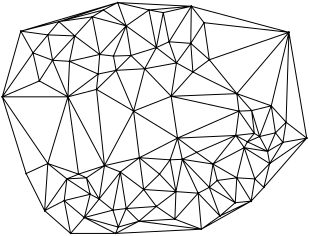
\includegraphics[width=\textwidth]{delaunay-alpha-a}
      \subcaption{Delaunay Triangulation einer beliebigen Punktmenge}
      \label{fig:delaunay-alpha-a}
    \end{subfigure}
    \hfill
    \begin{subfigure}[t]{\subwidth}
      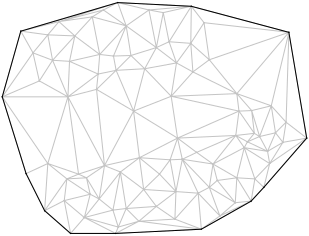
\includegraphics[width=\textwidth]{delaunay-alpha-b}
      \subcaption{Konvexe Hülle: Hülle der Triangulation}
      \label{fig:delaunay-alpha-b}
    \end{subfigure}
  }
  \vspace{2em}
  \captionsetup[subfigure]{singlelinecheck=false}{
    \def\subwidth{0.4\textwidth}
    \def\svgwidth{\textwidth}
    \begin{subfigure}[t]{\subwidth}
      \includegraphics[width=\textwidth]{delaunay-alpha-c}
      \subcaption{Alpha-Form: Hülle nach Entfernung von Simplexen mit $r_d > \alpha$}
      \label{fig:delaunay-alpha-c}
    \end{subfigure}
    \hfill
    \begin{subfigure}[t]{\subwidth}
      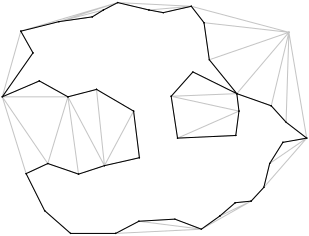
\includegraphics[width=\textwidth]{delaunay-alpha-d}
      \subcaption{Alpha-Form: Hülle nach Entfernung von Simplexen mit $r_d < \alpha$ (nur innen)}
      \label{fig:delaunay-alpha-c}
    \end{subfigure}
  }
  \caption[Methoden zur Bestimmung der Oberfläche per Delaunay-Triangulation]{Verschiedene Methoden zur Bestimmung der Oberfläche per Delaunay-Triangulation. Man beachte, dass die in (d) genutzte Methode den Ausreißer-Punkt oben rechts mit trianguliert, jedoch nicht zur Oberfläche zählt, da für keinen seiner Simplexe $r_d < \alpha$ gilt}
  \label{fig:delaunay-alpha}
\end{figure}
